% Turkish version of main.tex (SIU requires Turkish for native speakers; Özetçe + Abstract).
% Tables: paper/tables_tr (make_tables.py --lang tr); figures: *_tr.png (plot_results.py --lang tr, qualitative.py).
% Build: pdflatex main_tr && bibtex main_tr && pdflatex main_tr && pdflatex main_tr   (or: tectonic main_tr.tex)
\documentclass[conference]{IEEEtran}
\usepackage{iftex}
\ifXeTeX % tectonic / xelatex: Times clone; pdflatex (Overleaf) keeps IEEEtran's own Times
  \usepackage{fontspec}
  \setmainfont{texgyretermes}[Extension=.otf, UprightFont=*-regular, BoldFont=*-bold,
    ItalicFont=*-italic, BoldItalicFont=*-bolditalic]
\else
  \usepackage[T1]{fontenc}
  \usepackage[utf8]{inputenc}
\fi
\usepackage[turkish,shorthands=off]{babel}
\usepackage{graphicx}
\usepackage{booktabs}
\usepackage{amsmath}
\usepackage{hyperref}
\usepackage{xcolor}
\graphicspath{{figures/}}
\addto\captionsturkish{%
  \renewcommand{\abstractname}{Özetçe}%
  \renewcommand{\IEEEkeywordsname}{Anahtar Kelimeler}}
\newcommand{\nruns}{84}


\begin{document}

\title{Etiketler Kıt Olduğunda Yer Gözlem Temel Modelleri Sel Haritalamaya Ne Kadar Katkı Sağlar?\\
\large Prithvi-EO~2.0'ın Sen1Floods11 Üzerinde Donuk, LoRA ve Tam İnce Ayarı}

\author{\IEEEauthorblockN{Mert Semih Sar{\i}yerli}
\IEEEauthorblockA{Bilgisayar Mühendisliği Bölümü, Teknoloji Fakültesi\\
Gazi Üniversitesi, Ankara, Türkiye\\
semihmertsariyerli.06@gmail.com}}

\maketitle

\begin{abstract}
Yer gözlem temel modellerinin sel haritalama gibi görevler için gereken etiket sayısını azaltması beklenmektedir. Bu çalışmada söz konusu beklenti Sen1Floods11 veri kümesi üzerinde kontrollü bir düzenekte sınanmıştır. Sıfırdan ve ImageNet ağırlıklarıyla başlatılan iki U-Net, 300 milyon parametreli maskeli otokodlayıcı temel modeli Prithvi-EO~2.0 ile üç ince ayar rejiminde karşılaştırılmıştır: donuk kodlayıcı, düşük ranklı uyarlama (LoRA) ve tam ince ayar. Tüm modeller aynı altı Sentinel-2 bandını ve aynı optimizasyon adımı bütçesini kullanmış; eğitim etiketlerinin \%1'i ile \%100'ü (3 ile 252 karo) arasında, her ayar için üç rastgele tohumla toplam \nruns{} eğitim koşusu yapılmıştır. U-Net'ler her etiket oranında öndedir: tüm etiketlerle 0,829'a karşı LoRA'lı Prithvi'de 0,767 su IoU'su, yalnızca üç etiketli karoyla ise 0,809'a karşı 0,704. Dolayısıyla etiketler azaldıkça aradaki fark kapanmamakta, açılmaktadır. İnce ayar rejimleri arasında LoRA, yaklaşık 140 kat daha az eğitilen parametreyle tam ince ayarla aynı başarıyı (0,767'ye karşı 0,770) verirken donuk kodlayıcı ikisinin yaklaşık yedi puan gerisinde kalmaktadır. Ön eğitim, eğitimde görülmeyen Bolivya bölgesindeki başarım düşüşünü de azaltmamaktadır. Piksel düzeyindeki hata analizi, temel modelin eksiğinin su kenarlarında ve 0,1\,km$^2$'den küçük su kütlelerinde yoğunlaştığını, bunun da 16 piksellik yama çözünürlüğüyle tutarlı olduğunu göstermektedir. Bu veri kümesinde Sentinel-2 ile sel haritalama için, birkaç etiketli sahne olsa bile, küçük ve iyi ayarlanmış bir evrişimli ağ daha iyi bir seçenek olmayı sürdürmektedir.
\end{abstract}

\begin{IEEEkeywords}
sel haritalama, Sentinel-2, temel modeller, parametre-verimli ince ayar, LoRA, Sen1Floods11, alan kayması
\end{IEEEkeywords}

\begingroup
\renewcommand{\abstractname}{Abstract}
\renewcommand{\IEEEkeywordsname}{Keywords}
\begin{abstract}
Earth-observation foundation models are expected to reduce the number of labels needed for flood mapping. We test this on Sen1Floods11 by comparing two U-Nets (scratch and ImageNet-initialized) with Prithvi-EO~2.0 under frozen, LoRA and full fine-tuning, using the same six Sentinel-2 bands, the same optimizer-step budget, 1\,\%--100\,\% of the training labels and three seeds (\nruns{} runs). The U-Nets lead at every label fraction (0.829 vs.\ 0.767 water IoU at full labels, 0.809 vs.\ 0.704 with three labeled chips), so the gap widens as labels become scarce. LoRA matches full fine-tuning with about 140$\times$ fewer trainable parameters, and pretraining does not reduce the accuracy drop on the held-out Bolivia region. A pixel-level error analysis locates the foundation model's shortfall at water edges and on water bodies below 0.1\,km$^2$, consistent with its 16-pixel patch resolution.
\end{abstract}
\begin{IEEEkeywords}
flood mapping, Sentinel-2, foundation models, parameter-efficient fine-tuning, LoRA, Sen1Floods11, domain shift
\end{IEEEkeywords}
\endgroup

\section{Giriş}
Optik uydu görüntülerinden hızlı sel alanı haritalamayı model kapasitesinden çok piksel düzeyinde etiketlemenin maliyeti sınırlamaktadır: bu alandaki standart veri kümesi olan Sen1Floods11~\cite{bonafilia2020sen1floods11} yalnızca 446 elle etiketlenmiş karo içerir. Prithvi-EO~2.0~\cite{szwarcman2024prithvi} gibi yer gözlem (YG) temel modelleri, büyük etiketsiz arşivler üzerinde maskeli otokodlama ile ön eğitildikleri için etikete olan bu bağımlılığı azaltmayı vaat eder. Elinde birkaç etiketli sahne ve tek bir GPU bulunan bir uygulayıcı için iki soru önemlidir:
\begin{enumerate}
  \item Temel model, iyi ayarlanmış bir U-Net'e göre ne kadar doğruluk kazandırır ve etiketler azaldıkça bu üstünlük büyür mü?
  \item Hangi ince ayar rejimi---eğitilen bir başlıkla donuk kodlayıcı, düşük ranklı bağdaştırıcılar (LoRA)~\cite{hu2021lora} ya da tam ince ayar---eğitilen parametre başına en iyi doğruluğu verir ve hangisi görülmemiş bir bölgeye en iyi genelleşir?
\end{enumerate}
Her iki soruyu da sabit bir deney matrisiyle yanıtlıyoruz. Dört model (iki U-Net ile donuk ve LoRA'lı Prithvi), eğitim karolarının \%100'ünden \%1'ine kadar altı etiket oranında ve her biri üç tohumla eğitilmiştir. Tam ince ayar ve bir dizi ablasyon deneyi tüm etiketlerle eklenmiştir. Her koşu aynı optimizasyon adımı bütçesini kullanır ve Sen1Floods11'in dağılım içi test bölümü ile eğitimde görülmeyen Bolivya bölgesi üzerinde değerlendirilir.

\textbf{Katkılar.} (i) Sıfırdan ve ImageNet ile başlatılan U-Net'lerin donuk, LoRA ve tam ince ayarlı Prithvi-EO~2.0 ile Sen1Floods11 üzerinde, eşit adım bütçesiyle ve üç etiketli karoya kadar kontrollü karşılaştırması. (ii) Bu veri kümesinde temel modelin dezavantajının etiketler azaldıkça küçülmek yerine büyüdüğüne ve ön eğitimin görülmeyen bölgedeki düşüşü azaltmadığına dair kanıt. (iii) Temel modelin fazladan hatalarını su kenarlarına ve küçük su kütlelerine yerleştiren piksel düzeyinde bir hata analizi. (iv) Her koşunun yapılandırmasını ve metriklerini içeren açık ve yeniden üretilebilir bir işlem hattı (\url{https://github.com/mertsemih/eo-foundation-flood}).

\section{İlgili Çalışmalar}
\textbf{Sen1Floods11 üzerinde sel haritalama.} Bonafilia ve ark.~\cite{bonafilia2020sen1floods11}, Sen1Floods11'i on bir sel olayına ait çakıştırılmış Sentinel-1 ve Sentinel-2 karoları, elle etiketlenmiş bir alt küme ve aktarımı sınamak için ayrılmış bir Bolivya olayıyla birlikte yayımlamıştır. Sabit bölümleri ve küçük boyutu, bu veri kümesini YG temel modelleri için yaygın bir alt görev hâline getirmiştir.

\textbf{YG temel modelleri.} Prithvi~\cite{jakubik2023prithvi} ve Prithvi-EO~2.0~\cite{szwarcman2024prithvi}, görü dönüştürücülerini~\cite{dosovitskiy2021vit} Uyumlaştırılmış Landsat--Sentinel (HLS) görüntüleri üzerinde maskeli otokodlayıcı~\cite{he2022mae} olarak ön eğitir. İlgili modeller arasında SatMAE~\cite{cong2022satmae} ve algılayıcıdan bağımsız DOFA~\cite{xiong2024dofa} sayılabilir. GEO-Bench~\cite{lacoste2023geobench} ve PANGAEA~\cite{marsocci2024pangaea} gibi karşılaştırma kümeleri bu modelleri çok sayıda görevde değerlendirir. Çalışmamıza en yakın olan PANGAEA, temel modellerin denetimli modelleri ``tutarlı biçimde geçemediğini'' bildirir. Sen1Floods11 üzerinde denetimli U-Net karşılaştırma modeli etiketlerin \%100'ünde, \%50'sinde ve \%10'unda Prithvi'nin üzerindedir (mIoU \%100'de 91,42'ye karşı 90,37, \%10'da 88,55'e karşı 86,28). PANGAEA donuk kodlayıcılar üzerinde sabit sayıda dönem boyunca bir kod çözücü eğitir ve \%10 etikette durur. Bu tabloyu üç yönde genişletiyoruz: donuk, LoRA ve tam ince ayarı karşılaştırıyor, optimizasyon adımı bütçesini etiket oranlarından bağımsız sabit tutuyor ve etiketlerin \%1'ine kadar iniyoruz.

\textbf{Parametre-verimli ince ayar.} Bağdaştırıcılar~\cite{houlsby2019adapters} ve LoRA~\cite{hu2021lora}, ön eğitilmiş ağırlıklar sabit kalırken az sayıda eklenmiş parametreyi eğitir. Kumar ve arkadaşları~\cite{kumar2022lpft}, tam ince ayarın ön eğitilmiş öznitelikleri bozabildiğini ve dağılım dışında doğrusal yoklamanın gerisinde kalabildiğini göstermiştir. Üç rejimi Bolivya bölgesinde karşılaştırmamızın gerekçesi budur.

\section{Veri}
\subsection{Sen1Floods11}
Sen1Floods11'in elle etiketlenmiş alt kümesini kullanıyoruz: on bir sel olayına ait, 10\,m çözünürlükte $512\times512$ piksellik 446 karo. Her karoda Sentinel-2 L1C (13 bant), Sentinel-1 GRD (VV, VH) ve piksel başına $\{-1, 0, 1\}$ etiketi (veri yok/bulut, su yok, su) bulunur. Resmî bölümlemeyi izliyoruz: on bölgeden alınmış 252 eğitim, 89 doğrulama ve 90 test karosu; ayrıca başka hiçbir bölümde yer almayan ve dağılım dışı (DD) test olarak kullanılan 15 Bolivya karosu.

Verinin iki özelliği değerlendirmeyi biçimlendirir. Birincisi, su nadirdir: geçerli pikseller içinde ortanca karonun su oranı \%2,5'tir (eğitimde ortalama \%9); bu nedenle piksel doğruluğu yerine su IoU'su raporlanır. İkincisi, Bolivya bölümü yalnızca yeni bir bölge değil, aynı zamanda daha bulutludur: piksellerinin ortalama \%27'sinde veri yoktur, diğer bölümlerde bu oran \%13'tür. Bu nedenle her DD iddiası coğrafi kaymayla bulut örtüsü kaymasını birlikte içerir; bu konuya Bölüm~\ref{sec:discussion}'da dönüyoruz.

\subsection{Girdiler ve ön işleme}
Tüm modeller aynı altı Sentinel-2 bandını (B2, B3, B4, B8A, B11, B12) alır; bunlar Prithvi-EO'nun ön eğitildiği altı HLS bandına karşılık gelir. U-Net'leri aynı bantlarla sınırlamak, ön eğitimin etkisini girdi bilgisinin etkisinden ayırır. Yansıtım değerleri eğitim bölümünün istatistikleriyle bant başına standartlaştırılır. Eğitimde çevirme ve 90$^\circ$ döndürmeyle birlikte rastgele $224\times224$ kırpmalar, değerlendirmede ise $512\times512$ karoların tamamı kullanılır. $-1$ etiketli pikseller kayıp fonksiyonundan ve tüm metriklerden çıkarılır.

\subsection{Etiket oranı protokolü}
Her $f\in\{1;\ 0{,}25;\ 0{,}10;\ 0{,}05;\ 0{,}02;\ 0{,}01\}$ oranı için $\mathrm{yuvarla}(252 f)$ eğitim karosu tutulur; yani sırasıyla 252, 63, 25, 13, 5 ve 3 karo. Alt küme, koşunun tohumuyla belirlenen rastgele bir permütasyonla çekilir; böylece üç tohum hem başlatmayı hem de alt kümeyi değiştirir ve belirli bir tohum için her model aynı alt kümeyi görür. Doğrulama ve test kümeleri hiçbir zaman alt örneklenmez. Sabit bir dönem sayısıyla, düşük etiketli koşular orantılı olarak daha az parametre güncellemesi alırdı. Bu nedenle her koşu aynı öğrenme oranı çizelgesiyle yaklaşık 1550 optimizasyon adımlık aynı bütçe boyunca eğitilir. Dönemler tam koşulduğundan kesin sayı 1550--1575 adımdır: tüm etiketlerle 50 dönem, daha küçük yığın kullanan tam ince ayarda 25 dönem. $f\le0{,}02$ için yığın boyutu eğitim karosu sayısına indirilir.

\section{Yöntem}
\subsection{Karşılaştırma modelleri}
\textbf{U-Net (sıfırdan)}, rastgele başlatılarak eğitilen ve ResNet-34~\cite{he2016resnet} kodlayıcılı (24,4 milyon parametre) bir U-Net'tir~\cite{ronneberger2015unet}. \textbf{U-Net (ImageNet)}, aynı mimarinin ImageNet ile ön eğitilmiş kodlayıcılı hâlidir ve ``genel'' ile ``YG'ye özgü'' ön eğitimi karşılaştırmak için bir kontrol işlevi görür.

\subsection{Üç ince ayar rejimiyle Prithvi-EO 2.0}
Prithvi-EO~2.0~(300M), HLS görüntüleri üzerinde ön eğitilmiş bir ViT-L maskeli otokodlayıcıdır (24 blok, 1024 gömme boyutu, 16 yama boyutu). Kodlayıcının son dört bloğunun belirteç haritalarını birleştirip hafif, tam evrişimli bir başlıkla (dört üst örnekleme aşaması, 1,4 milyon parametre) çözüyoruz. Üç rejim yalnızca kodlayıcının hangi parametrelerinin gradyan aldığıyla ayrılır:
\begin{itemize}
  \item \textbf{Donuk}: kodlayıcı sabit, yalnızca başlık eğitilir (1,4 milyon eğitilen parametre).
  \item \textbf{LoRA}: her bloğun sorgu/anahtar/değer izdüşümlerine rank-8 bağdaştırıcılar ($\alpha=16$, bırakma oranı 0,05); 0,8 milyon bağdaştırıcı parametresi, toplamda 2,2 milyon eğitilen parametre.
  \item \textbf{Tam}: 305 milyon parametrenin tümü; kodlayıcının öğrenme oranı başlığınkinin 20'de biridir.
\end{itemize}

\subsection{Eğitim ve değerlendirme}
Tüm modellerde AdamW~\cite{loshchilov2019adamw}, doğrusal ısınmalı kosinüs öğrenme oranı çizelgesi, 1,0'da gradyan kırpma, karma hassasiyet ve ağırlıksız çapraz entropi kaybı kullanılır. Başlık (ya da U-Net'in tamamı) $10^{-3}$ öğrenme oranıyla eğitilir; ImageNet U-Net'inde bu değer $5\times10^{-4}$'tür. Bağdaştırıcılar LoRA'da başlık oranının 0,5 katını, kodlayıcı tam ince ayarda 0,05 katını kullanır. Ağırlık azaltma 0,01 (tam ince ayarda 0,05), ısınma 100 adım (tam ince ayarda 200) ve yığın boyutu 8'dir. Tam ince ayar, 8\,GB GPU belleğine sığmak için 4'lük yığın kullanır. Her koşu yaklaşık 50 kez (tam ince ayarda 25 kez) doğrulanır ve doğrulama su IoU'su en yüksek olan kontrol noktası test ve Bolivya bölümlerinde değerlendirilir. Su IoU'su, bir bölümün tüm geçerli pikselleri üzerinde biriktirilen karışıklık matrisinden hesaplanır. Üç tohum üzerinden ortalama $\pm$ standart sapma raporlanır. Tohum-0 koşuları tek bir RTX~3070~Ti dizüstü GPU'sunda (8\,GB), sonraki tohumların bir kısmı Colab T4 üzerinde çalıştırılmıştır. Çalışmanın tamamı 12,7 GPU-saat sürmüştür.

\section{Bulgular}
\subsection{Tüm etiketlerle}
Tablo~\ref{tab:full}, beş ana modeli $f=1$ için verir. Her iki U-Net de 0,82--0,83 test su IoU'suna ulaşır. En iyi Prithvi varyantları 0,767 (LoRA) ve 0,770 (tam ince ayar) ile yaklaşık altı puan geride, donuk kodlayıcı ise 0,701'dedir. Bir U-Net ile bir Prithvi varyantı arasındaki her fark, en fazla 0,015 olan tohum standart sapmalarının birkaç katıdır. ImageNet ile başlatma, sıfırdan eğitime göre 0,6 puan ekler; bu fark tohum yayılımının içindedir.

\begin{table}[t]
\centering
\caption{Tüm eğitim etiketleriyle ($f=1$) test ve eğitimde görülmeyen Bolivya bölümlerinde su IoU'su; üç tohum üzerinden ortalama $\pm$ std. GPU dakikaları, RTX~3070~Ti (8\,GB) üzerindeki tohum-0 koşusuna aittir.}
\label{tab:full}
\resizebox{\columnwidth}{!}{\begin{tabular}{llrrrr}
\toprule
Model & Ön eğitim & Eğitilen & Test IoU$_s$ & Bolivya IoU$_s$ & GPU dk \\
\midrule
U-Net (sıfırdan) & -- & 24,4\,M & 0,823 $\pm$ 0,008 & 0,766 $\pm$ 0,021 & 3,9 \\
U-Net (ImageNet) & ImageNet & 24,4\,M & \textbf{0,829 $\pm$ 0,015} & \textbf{0,781 $\pm$ 0,007} & 3,7 \\
Prithvi donuk & Prithvi-EO 2.0 & 1,4\,M & 0,701 $\pm$ 0,005 & 0,606 $\pm$ 0,083 & 8,7 \\
Prithvi LoRA (r=8) & Prithvi-EO 2.0 & 2,2\,M & 0,767 $\pm$ 0,011 & 0,717 $\pm$ 0,019 & 13,3 \\
Prithvi tam ince ayar & Prithvi-EO 2.0 & 305\,M & 0,770 $\pm$ 0,010 & 0,695 $\pm$ 0,050 & 9,0 \\
\bottomrule
\end{tabular}
}
\end{table}

\begin{figure*}[t]
\centering
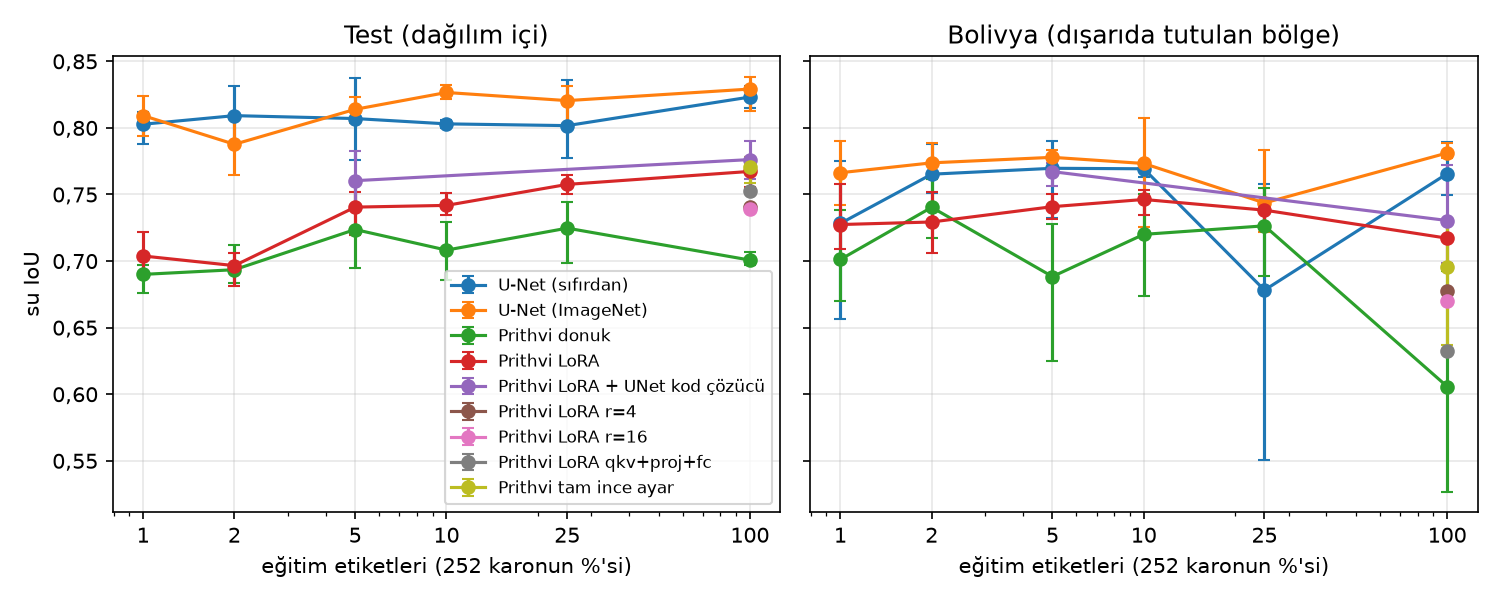
\includegraphics[width=0.95\textwidth]{fig1_iou_vs_labels_tr.png}
\caption{Eğitim etiketi oranına göre su IoU'su (logaritmik ölçek; \%100 = 252 karo): test bölümü (sol) ve eğitimde görülmeyen Bolivya bölgesi (sağ). İşaretler üç tohumun ortalamasını, hata çubukları aralığı (en küçük--en büyük) gösterir. Çizgisiz noktalar yalnızca $f=1$'de koşulan yapılandırmalardır (tam ince ayar ile LoRA rank/hedef ablasyonları); çok ölçekli kod çözücü \%5 ve \%100'de koşulmuştur.}
\label{fig:labels}
\end{figure*}

\begin{table}[t]
\centering
\caption{Eğitim etiketi oranına göre test su IoU'su (parantez içinde karo sayısı), üç tohum üzerinden ortalama $\pm$ std. Her satırın en iyisi kalın.}
\label{tab:sweep}
\resizebox{\columnwidth}{!}{\begin{tabular}{lrrrr}
\toprule
Etiket & U-Net (sıfırdan) & U-Net (ImageNet) & Prithvi donuk & Prithvi LoRA (r=8) \\
\midrule
\%100 (252) & 0,823 $\pm$ 0,008 & \textbf{0,829 $\pm$ 0,015} & 0,701 $\pm$ 0,005 & 0,767 $\pm$ 0,011 \\
\%25 (63) & 0,802 $\pm$ 0,031 & \textbf{0,820 $\pm$ 0,016} & 0,725 $\pm$ 0,024 & 0,758 $\pm$ 0,007 \\
\%10 (25) & 0,803 $\pm$ 0,003 & \textbf{0,827 $\pm$ 0,005} & 0,708 $\pm$ 0,022 & 0,742 $\pm$ 0,009 \\
\%5 (13) & 0,807 $\pm$ 0,031 & \textbf{0,814 $\pm$ 0,010} & 0,724 $\pm$ 0,034 & 0,741 $\pm$ 0,018 \\
\%2 (5) & \textbf{0,809 $\pm$ 0,022} & 0,788 $\pm$ 0,021 & 0,694 $\pm$ 0,016 & 0,697 $\pm$ 0,013 \\
\%1 (3) & 0,803 $\pm$ 0,013 & \textbf{0,809 $\pm$ 0,015} & 0,690 $\pm$ 0,012 & 0,704 $\pm$ 0,017 \\
\bottomrule
\end{tabular}
}
\end{table}

\begin{table}[t]
\centering
\caption{Eğitim etiketi oranına göre Bolivya (eğitimde görülmeyen bölge) su IoU'su.}
\label{tab:sweep_bolivia}
\resizebox{\columnwidth}{!}{\begin{tabular}{lrrrr}
\toprule
Etiket & U-Net (sıfırdan) & U-Net (ImageNet) & Prithvi donuk & Prithvi LoRA (r=8) \\
\midrule
\%100 (252) & 0,766 $\pm$ 0,021 & \textbf{0,781 $\pm$ 0,007} & 0,606 $\pm$ 0,083 & 0,717 $\pm$ 0,019 \\
\%25 (63) & 0,678 $\pm$ 0,112 & \textbf{0,744 $\pm$ 0,035} & 0,726 $\pm$ 0,034 & 0,738 $\pm$ 0,010 \\
\%10 (25) & 0,769 $\pm$ 0,006 & \textbf{0,773 $\pm$ 0,043} & 0,720 $\pm$ 0,041 & 0,746 $\pm$ 0,010 \\
\%5 (13) & 0,770 $\pm$ 0,032 & \textbf{0,778 $\pm$ 0,008} & 0,688 $\pm$ 0,055 & 0,741 $\pm$ 0,009 \\
\%2 (5) & 0,765 $\pm$ 0,020 & \textbf{0,774 $\pm$ 0,014} & 0,740 $\pm$ 0,022 & 0,729 $\pm$ 0,023 \\
\%1 (3) & 0,728 $\pm$ 0,063 & \textbf{0,766 $\pm$ 0,024} & 0,701 $\pm$ 0,034 & 0,727 $\pm$ 0,027 \\
\bottomrule
\end{tabular}
}
\end{table}

\subsection{Az etiketle}
Şekil~\ref{fig:labels} ve Tablo~\ref{tab:sweep} etiket taramasını gösterir. Test bölümünde hiçbir U-Net eğrisi bir Prithvi eğrisiyle kesişmez. Etiketlerin \%100'ünden \%1'ine inildiğinde her iki U-Net de yaklaşık iki puan kaybeder (0,829$\to$0,809 ve 0,823$\to$0,803); üç etiketli karoyla bile tüm etiketlerle eğitilmiş LoRA'nın üzerindedirler. LoRA'lı Prithvi aynı aralıkta altı puan kaybeder (0,767$\to$0,704). Donuk kodlayıcı, öznitelikleri uyarlanmayan bir modelden beklendiği gibi 0,69 ile 0,73 arasında düz seyreder. Daha iyi U-Net ile LoRA arasındaki fark \%100'de 6,2, \%5'te 7,3, \%2'de 11,3 ve \%1'de 10,5 puandır. Artış tekdüze değildir, ancak etiketler azaldıkça fark yaklaşık altı puandan yaklaşık on bir puana çıkar. Tablo~\ref{tab:sweep}'deki her U-Net ortalaması en az 0,788, her Prithvi ortalaması ise en fazla 0,767'dir.

\%1--2 etiket oranlarında tohum alt kümeyi de değiştirir. Dolayısıyla tohumlar arasındaki yayılım (U-Net'lerde en fazla 0,022) hangi karoların çekildiğinin etkisini de içerir ve yine de model aileleri arasındaki farkın çok altında kalır.

\subsection{Eğitilen parametre başına doğruluk}
\begin{figure}[t]
\centering
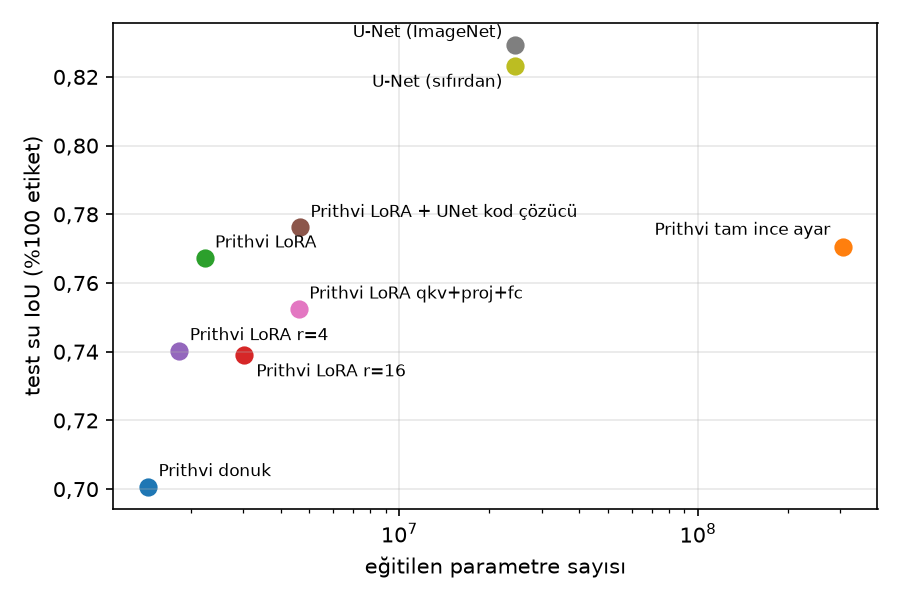
\includegraphics[width=\columnwidth]{fig3_iou_vs_params_tr.png}
\caption{$f=1$'de eğitilen parametre sayısına (logaritmik ölçek) göre test su IoU'su.}
\label{fig:params}
\end{figure}
Şekil~\ref{fig:params} her yapılandırmayı eğitilen parametre sayısına göre konumlandırır. LoRA, tam ince ayarın güncellediği 305 milyon parametrenin \%0,7'si olan 2,2 milyon parametreyi eğitir ve aynı test doğruluğuna ulaşır (0,767 $\pm$ 0,011'e karşı 0,770 $\pm$ 0,010; yani \%99,6'sı). Donuk kodlayıcıya 0,8 milyon bağdaştırıcı parametresi eklemek 6,7 puan kazandırır. Bunun ötesinde ne daha fazla bağdaştırıcı kapasitesi ne de yaklaşık 140 kat daha fazla eğitilen parametre Prithvi'yi iyileştirir; hiçbiri 24 milyon parametreli U-Net'lerle arasındaki farkı kapatmaz.

\subsection{Bolivya'ya aktarım}
\begin{figure}[t]
\centering
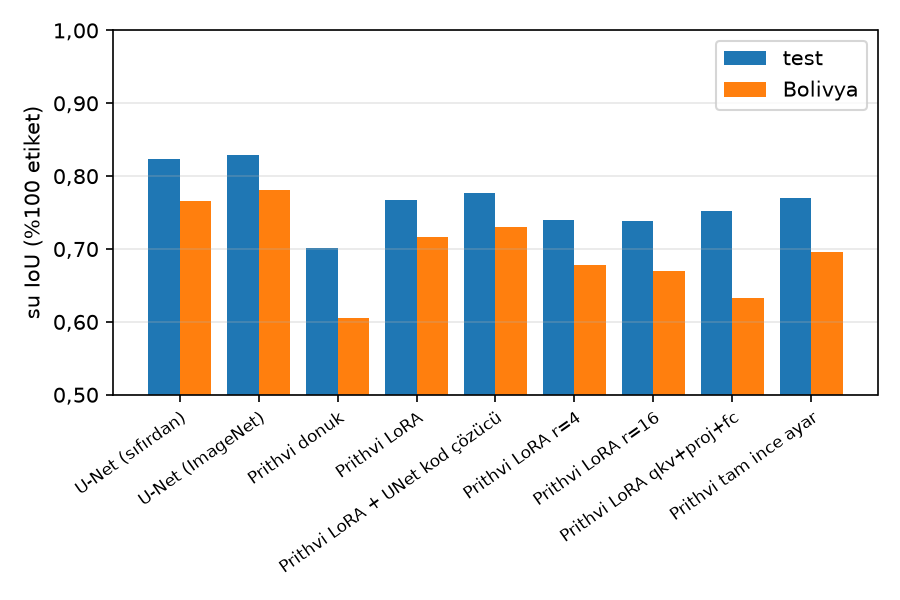
\includegraphics[width=\columnwidth]{fig2_ood_gap_tr.png}
\caption{Her yapılandırma için $f=1$'de test ve Bolivya su IoU'su.}
\label{fig:ood}
\end{figure}
Tüm modeller Bolivya'da doğruluk kaybeder (Şekil~\ref{fig:ood}). $f=1$'de testten Bolivya'ya düşüş ImageNet U-Net'i için 4,8, sıfırdan U-Net için 5,8, LoRA için 5,0, tam ince ayar için 7,5 ve donuk kodlayıcı için 9,5 puandır. Dolayısıyla YG ön eğitimi aktarım açığını küçültmez. ImageNet U-Net'i her etiket oranında en yüksek Bolivya doğruluğuna sahiptir (Tablo~\ref{tab:sweep_bolivia}) ve beş ana model arasında en küçük düşüşü gösterir. LoRA'nın Bolivya skoru (0,717 $\pm$ 0,019) tam ince ayarınkinin (0,695 $\pm$ 0,050) üzerindedir. Bu, Kumar ve arkadaşlarının~\cite{kumar2022lpft} gözlemiyle tutarlıdır; ancak fark tam ince ayarın yayılımı içinde kaldığından kesin değildir.

Bolivya sonuçları test sonuçlarından daha gürültülüdür. \%25 etiketle sıfırdan U-Net'in bir tohumu 0,55'tir (std 0,112) ve LoRA'nın Bolivya skoru etiket oranıyla tekdüze değişmez: \%10'daki 0,746, \%100'deki 0,717'den yüksektir. Dörtte biri veri yok piksellerinden oluşan 15 karoluk bu bölüm, model ailelerini güvenilir biçimde sıralar, ancak birbirine yakın yapılandırmaları sıralayamaz.

\subsection{Ablasyon}
\begin{table}[t]
\centering
\caption{$f=1$'de ablasyonlar: LoRA rankı, LoRA hedef modülleri ve kod çözücü ($\dagger$: tek tohum).}
\label{tab:ablation}
\resizebox{\columnwidth}{!}{\begin{tabular}{lrrr}
\toprule
Varyant & Eğitilen & Test IoU$_s$ & Bolivya IoU$_s$ \\
\midrule
LoRA r=4, qkv & 1,83\,M & 0,740$^\dagger$ & 0,678$^\dagger$ \\
LoRA r=8, qkv (ana) & 2,23\,M & 0,767 $\pm$ 0,011 & 0,717 $\pm$ 0,019 \\
LoRA r=16, qkv & 3,01\,M & 0,739$^\dagger$ & 0,670$^\dagger$ \\
LoRA r=8, qkv+proj+fc1+fc2 & 4,61\,M & 0,752$^\dagger$ & 0,632$^\dagger$ \\
LoRA r=8, qkv + çok ölçekli UNet kod çözücü & 4,65\,M & 0,776 $\pm$ 0,014 & 0,730 $\pm$ 0,038 \\
\bottomrule
\end{tabular}
}
\end{table}
Tablo~\ref{tab:ablation} LoRA yapılandırmasını değiştirir. 4, 8 ve 16 rankları arasında sorgu/anahtar/değer izdüşümlerindeki rank~8 en iyi tohum-0 sonucunu vermiştir (0,740; 0,778 ve 0,739; rank~8 için üç tohum üzerinden 0,767 $\pm$ 0,011). Bağdaştırıcıları dikkat çıkışı ve MLP katmanlarına da eklemek eğitilen parametreleri iki katına çıkarır ve Bolivya skorunu 0,632'ye düşürür. Tek tohumlu bu üç-dört puanlık farklar yalnızca yol gösterici niteliktedir.

Hafif başlığın Prithvi'yi sınırlayıp sınırlamadığını sınamak için başlığı 6, 12, 18 ve 24. blokların çıktıları üzerinde çalışan çok ölçekli, U-Net tarzı bir kod çözücüyle (4,65 milyon eğitilen parametre) değiştirdik. Üç tohum üzerinden bu kod çözücü $f=1$'de 0,776 $\pm$ 0,014 (FCN başlığıyla gürültü sınırları içinde eşit) ve \%5'te 0,760 $\pm$ 0,022 (FCN başlığı: 0,741 $\pm$ 0,018) değerine ulaşır. Daha güçlü bir kod çözücü etiketler kıtken az da olsa yardımcı olur, ancak U-Net'lerle arada yaklaşık beş puanlık fark bırakır. Dolayısıyla bu görevdeki eksiklik başlıkta değil, kodlayıcının temsilindedir.

\subsection{Hataların yeri}
\begin{figure*}[t]
\centering
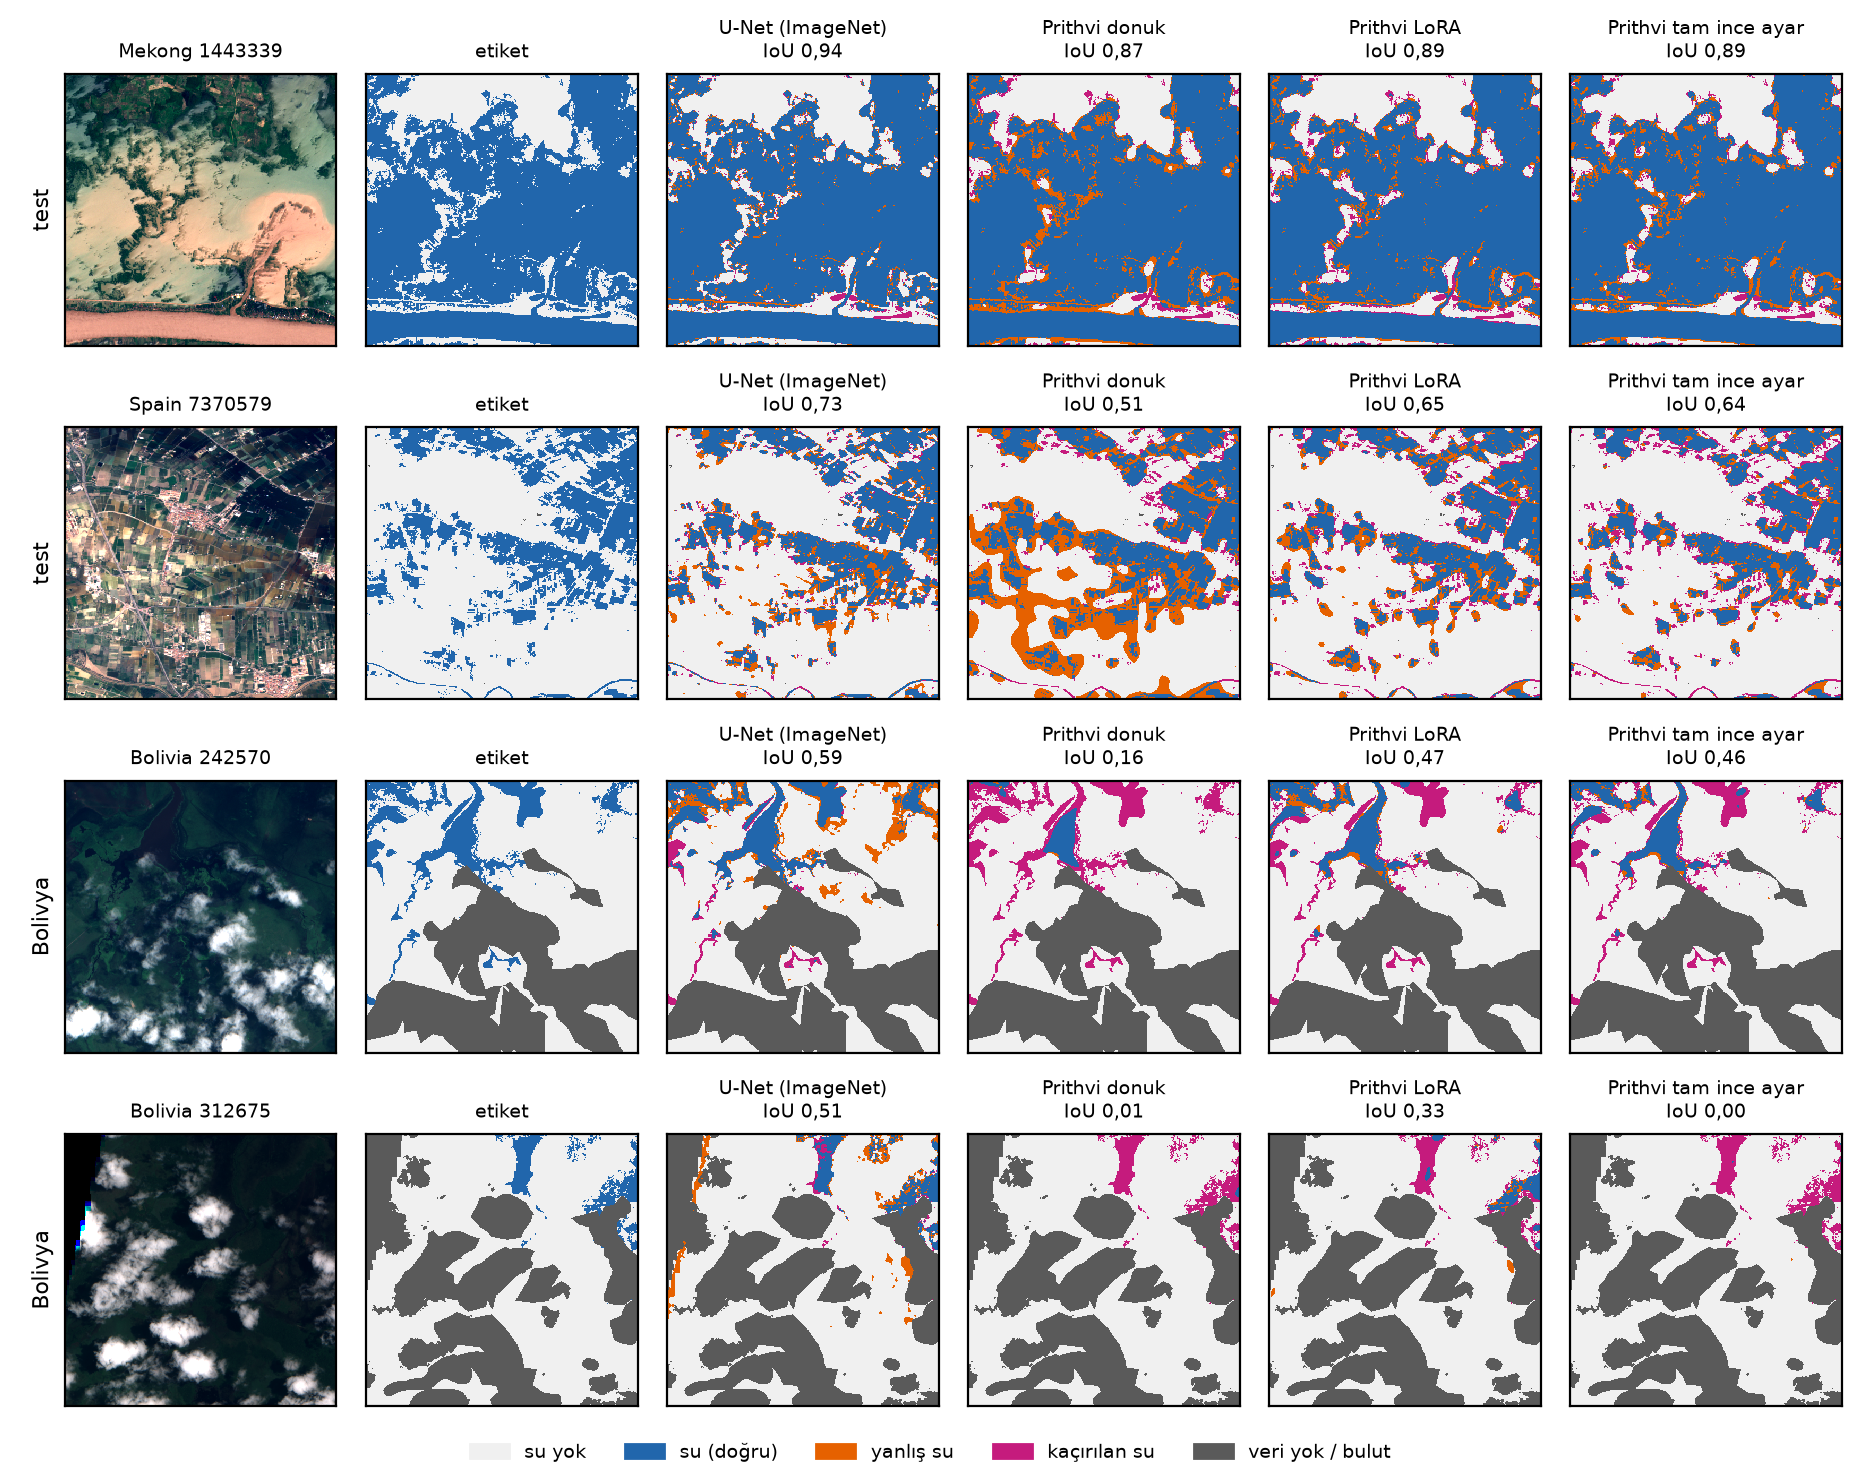
\includegraphics[width=\textwidth]{fig4_predictions_tr.png}
\caption{Tüm etiketlerle eğitilmiş tohum-0 modellerinin tahminleri, elle yapılmış etikete göre hata haritası olarak. Satırlar gözle değil sabit bir kuralla seçilmiştir: en az \%5 su içeren karolar arasından, ImageNet U-Net'i ile LoRA'lı Prithvi arasındaki karo başına IoU farkının 50. ve 75. yüzdelik dilimindeki karolar; üstte test bölümü, altta Bolivya. Başlıklar karo başına su IoU'sunu verir.}
\label{fig:pred}
\end{figure*}
Toplu sayıların gizlediklerini görmek için tüm test ve Bolivya karolarını $f=1$'deki tohum-0 kontrol noktalarıyla tahmin edip hataları piksel piksel inceledik. Şekil~\ref{fig:pred} sabit bir kuralla seçilmiş dört karoyu gösterir. İki örüntü göze çarpar. Birincisi, Prithvi U-Net'in yakaladığı dar kanalları ve küçük gölcükleri kaçırır; İspanya karosunun altındaki nehir buna bir örnektir. İkincisi, su sınırlarını etiketten daha pürüzsüz çizer ve kenarlar boyunca yanlış ve kaçırılmış su şeritleri oluşur. Bolivya'da Prithvi varyantları suyun önemli bir kısmını kaçırır (bölüm genelinde duyarlılık 0,53--0,77, U-Net'lerde 0,83--0,89), U-Net ise bir miktar yanlış su ekler.

Test bölümünde iki ölçüm bu örüntüleri sayısallaştırır; denediğimiz eşiklere karşı sağlamdırlar. \emph{Su kütlesi boyutu:} etiketlenmiş suyu bağlantılı bileşenlere ayırdık. 1000 pikselden (0,1\,km$^2$) küçük su kütleleri su piksellerinin \%11'ini içerir. Bunlarda duyarlılık U-Net'ler için 0,68--0,69, Prithvi için ise 0,48 (LoRA) ve 0,43'tür (tam). Daha büyük kütlelerde U-Net'ler ve ince ayarlı Prithvi varyantları 0,90--0,93'e ulaşır. Aynı sıralama 500 ve 2000 piksellik eşiklerde de geçerlidir. \emph{Kenarlar:} Prithvi'nin hatalarının \%77'si etiketteki su kenarına en fazla 3 piksel uzaklıktadır; U-Net'lerde bu oran \%64--65'tir. Mutlak sayılarla LoRA kenarların yakınında 484 bin hatalı piksel yaparken U-Net'ler 319--342 bin yapar; kenarlardan uzakta ise LoRA daha az hata yapar (144 bine karşı 172--192 bin). Yani Prithvi'nin fazladan hatalarının tamamı su sınırlarında toplanır. Kenara 1 piksel mesafede hata payları tüm modellerde eşittir (\%44--46); fark kenardan 2--5 piksel uzakta ortaya çıkar. Dolayısıyla Prithvi kenar piksellerinin kendisinde başarısız olmaktan çok sınırları birkaç piksel kaydırır. Kesinliği U-Net'lerle aynı düzeydedir (0,89--0,91); kaybedilen doğruluk duyarlılıktadır (0,89--0,90'a karşı 0,85--0,86).

\section{Tartışma}
\label{sec:discussion}
\textbf{İddiaların yeniden değerlendirilmesi.} Deneylerden önce şunları bekliyorduk: (1) tüm etiketlerle temel model için en fazla marjinal bir üstünlük, (2) \%5--10 etikette büyüyen bir üstünlük, (3) LoRA'nın parametrelerin küçük bir kısmıyla tam ince ayarın büyük bölümünü yakalaması ve (4) ön eğitimin Bolivya'da dağılım içine göre daha çok yardımcı olması. (1) numaralı iddia geçerlidir, ancak ters yönde: U-Net'ler altı puan öndedir. (2) numaralı iddia \%1'e kadar çürütülmüştür; fark en çok \%1--2'de açılır (10,5--11,3 puan). (3) numaralı iddia doğrulanmıştır; LoRA tam ince ayarı tamamen yakalar. (4) numaralı iddia çürütülmüştür: ana modeller arasında en iyi aktarımı ImageNet U-Net'i yapar.

\textbf{U-Net neden üç karoyla bile yetişiyor?} Bölütleme etiketleri yoğundur. $512\times512$'lik bir karo 262 bine kadar etiketli piksel sağlar ve üç karo $10^5$ mertebesinde su pikseli içerebilir. Yerel alıcı alanlara ve tam çözünürlüklü atlama bağlantılarına sahip bir evrişimli ağ için bu, özellikle adım bütçesi sabit tutulduğunda önemli bir eğitim sinyalidir. Sonuçlarımız, farklı bir protokolle U-Net'i Sen1Floods11 üzerinde \%10 etikete kadar Prithvi'nin önünde bulan PANGAEA~\cite{marsocci2024pangaea} ile uyumludur.

\textbf{Prithvi neden geride kalıyor?} Hata analizi uzamsal çözünürlüğe işaret eder. ViT görüntüyü $16\times16$'lık yamalar olarak görür; dolayısıyla öznitelikleri girdi çözünürlüğünün 1/16'sındadır. Fazladan hataları tam da bunun zarar vermesi beklenen yerlerdedir: su kenarları boyunca ve 0,1\,km$^2$'den küçük su kütlelerinde. Büyük su kütlelerinde U-Net kadar doğrudur ve kenarlardan uzakta daha az hata yapar. Çok ölçekli kod çözücü farkı kapatmaz, çünkü tüm girdileri aynı 1/16 çözünürlüklü belirteç ızgarasından gelir; tam çözünürlüklü girdiden bir atlama bağlantısı içeren kod çözücü bir sonraki doğal sınama olacaktır. Sınanmamış ikinci bir etken girdi alanıdır: Prithvi 30\,m HLS yüzey yansıtımı üzerinde ön eğitilmiştir, Sen1Floods11 ise 10\,m Sentinel-2 atmosfer üstü (L1C) yansıtım sağlar.

\textbf{Bolivya karıştırıcısı.} Bolivya karoları hem yeni bir bölgeden hem de daha bulutlu olduğundan, ölçtüğümüz düşüş coğrafi kaymayla eksik veriyi birlikte içerir. İkisini ayırmak bulut oranı eşleştirilmiş bir DD bölümü gerektirir. Bölümün küçüklüğü de modellerin ne kadar ince sıralanabileceğini sınırlar. Bu nedenle yalnızca hiçbir YG ön eğitimli modelin ImageNet U-Net'inden belirgin biçimde daha iyi aktarım yapmadığını söylüyoruz.

\textbf{Uygulayıcıya öneri.} Birkaç etiketli Sentinel-2 sel sahnesi ve tek bir tüketici GPU'su olan bir uygulayıcı için ImageNet ile başlatılmış bir U-Net, sınadığımız en doğru seçenektir. Koşu başına yaklaşık 4 GPU-dakika ile, Prithvi'nin 9--13 dakikasına karşı en ucuzudur da. Bir temel model gerekliyse (örneğin başka görevlerle tutarlılık için), LoRA eğitilen parametrelerin \%1'inden azıyla ve birkaç megabaytlık kontrol noktalarıyla tam ince ayar doğruluğu sağlar.

\section{Sınırlılıklar}
Çalışma tek bir veri kümesini ve algılayıcıyı (yalnızca Sentinel-2, SAR füzyonu yok) ve tek boyutta tek bir temel modeli kapsar. Hiperparametreler etiket oranına göre ayarlanmamıştır; tüketici GPU bütçesi de tam ince ayarı 4'lük yığınla sınırlar; bu yüzden tam ince ayar aynı adım bütçesinde diğer modellerin yarısı kadar örnek görür. Bolivya DD bölümü küçüktür (15 karo) ve diğerlerinden daha bulutludur. LoRA rankı ve hedef ablasyonları ile piksel düzeyindeki hata analizi tek tohum kullanır. Mutlak sayılar, farklı bant kümeleri, kod çözücüler ve eğitim bütçeleri kullanan diğer Prithvi sonuçlarıyla~\cite{szwarcman2024prithvi} karşılaştırılamaz; iddialarımız eşleştirilmiş bir protokol altındaki göreli sıralamaya ilişkindir.

\section{Sonuç}
Sentinel-2 girdisi ve eşit eğitim bütçesiyle Sen1Floods11 üzerinde U-Net'ler Prithvi-EO~2.0'ı tüm etiketlerle altı, üç etiketli karoyla on puan geçmektedir. Temel modelin az etiketli rejimde beklenen üstünlüğü ortaya çıkmamış, ön eğitim görülmeyen bir bölgedeki doğruluk kaybını da azaltmamıştır. Modelin fazladan hataları su kenarlarında ve küçük su kütlelerindedir; bu da sınırlayıcı etken olarak 16 piksellik yama çözünürlüğüne işaret etmektedir. Temel model ailesi içinde tercih edilecek rejim LoRA'dır: eğitilen parametrelerin yaklaşık 140'ta biriyle tam ince ayarla aynı başarıyı verir.

\section*{Yeniden Üretilebilirlik}
Kod, yapılandırmalar ve koşu başına metrikler \url{https://github.com/mertsemih/eo-foundation-flood} adresindedir. Her koşu tek bir YAML dosyasıyla tümüyle tanımlanır; veri kümesi, herkese açık Sen1Floods11 deposundan tek bir betikle indirilir.

\bibliographystyle{IEEEtran}
\bibliography{refs}

\end{document}
